% =====================================================================
%  Neural Morphogen Operators -- FULL version (archival / arXiv).
%
%  This file and workshop.tex assemble the same sources under sections/.
%  Nothing is duplicated between them, so a correction to a claim lands in
%  both builds and the two cannot drift apart -- which is the entire point
%  of not forking the manuscript for the shorter venue.
%
%  Length is controlled by the \fullpaper switch, which the section sources
%  read to drop material the short build has no room for.
% =====================================================================
\newif\iffullpaper
\fullpapertrue

\documentclass{article}

% NeurIPS 2026 style. Use [final] for the camera-ready, [preprint] for arXiv.
\usepackage{neurips_2026}

\usepackage[utf8]{inputenc}
\usepackage[T1]{fontenc}
\usepackage{hyperref}
\usepackage{url}
\usepackage{booktabs}
\usepackage{amsfonts}
\usepackage{amsmath}
\usepackage{amssymb}
\usepackage{nicefrac}
\usepackage{microtype}
\usepackage{graphicx}
\usepackage{subcaption}
\usepackage{xcolor}
\usepackage{amsthm}
\usepackage{mathtools}
\usepackage{bm}

\theoremstyle{plain}
\newtheorem{theorem}{Theorem}
\newtheorem{proposition}[theorem]{Proposition}
\newtheorem{lemma}[theorem]{Lemma}
\newtheorem{corollary}[theorem]{Corollary}
\theoremstyle{definition}
\newtheorem{definition}[theorem]{Definition}
\newtheorem{assumption}[theorem]{Assumption}
\theoremstyle{remark}
\newtheorem{remark}[theorem]{Remark}

\hypersetup{colorlinks=true, linkcolor=black, citecolor=black, urlcolor=blue!60!black}

% Auto-generated numbers (src/evaluation/numbers.py). Never edit by hand.
% Every result quoted inline is a macro defined there, so the prose cannot
% drift from the experiments. Missing runs expand to a visible ??.
\IfFileExists{numbers.tex}{% Auto-generated by src/evaluation/numbers.py -- do not edit by hand.
\providecommand{\NA}{\textbf{??}}
\newcommand{\NMOPearson}{\ensuremath{0.247 \pm 0.005}}
\newcommand{\NMORMSE}{\ensuremath{0.252 \pm 0.004}}
\newcommand{\NMOSSIM}{\ensuremath{0.404 \pm 0.006}}
\newcommand{\NMOMoran}{\ensuremath{0.762 \pm 0.004}}
\newcommand{\NMOParams}{2.20M}
\newcommand{\NSeeds}{3}
\newcommand{\BestBaseline}{spagcn}
\newcommand{\BestBaselinePearson}{\ensuremath{0.234 \pm 0.001}}
\newcommand{\BestBaselineMoran}{\ensuremath{0.738 \pm 0.002}}
\newcommand{\BestBaselineSSIM}{\ensuremath{0.393 \pm 0.001}}
\newcommand{\BestAnySSIM}{0.394}
\newcommand{\BestAnySSIMModel}{stagate}
\newcommand{\BestAnyMoran}{0.720}
\newcommand{\BestAnyMoranModel}{gp}
\newcommand{\SSIMDelta}{0.010}
\newcommand{\MoranDelta}{0.042}
\newcommand{\PearsonGain}{0.013}
\newcommand{\PearsonGainPct}{5.4}
\newcommand{\AEPearson}{0.230}
\newcommand{\BestGraphOverAE}{0.005}
\newcommand{\WorstGraphOverAE}{-0.002}
\newcommand{\NGraphBelowAE}{1}
\newcommand{\NGraphModels}{4}
\newcommand{\NMOOverAE}{0.017}
\newcommand{\NMOvsGraphRatio}{3.6}
\newcommand{\NMOMoranPred}{\ensuremath{0.936 \pm 0.004}}
\newcommand{\MoranTrue}{\ensuremath{0.174}}
\newcommand{\AblFull}{\ensuremath{\mathbf{??}}}
\newcommand{\AblNoDynamics}{0.227}
\newcommand{\AblNoDynamicsDelta}{\ensuremath{\mathbf{??}}}
\newcommand{\AblNoReaction}{0.227}
\newcommand{\AblNoReactionDelta}{\ensuremath{\mathbf{??}}}
\newcommand{\NDatasets}{6}
\newcommand{\NSections}{9}
\newcommand{\TotalLocations}{469{,}038}
}{\providecommand{\NA}{\textbf{??}}}

% Tables are generated by src/evaluation/tables.py. \inputtable degrades
% gracefully so a partial run yields a partial paper rather than a broken build.
\newcommand{\inputtable}[1]{%
  \IfFileExists{tables/#1.tex}{\input{tables/#1}}%
  {\begin{table}[t]\centering\small\textit{[table not yet generated -- run
     \texttt{make figures}]}\end{table}}}

% Any inline number whose run has not completed expands to ?? rather than to a
% stale value. These stubs are overwritten by numbers.tex when it exists.
\makeatletter
\@for\@nmocmd:={NMOPearson,NMORMSE,NMOSSIM,NMOMoran,NMOParams,NSeeds,BestBaseline,%
  BestBaselinePearson,BestBaselineMoran,PearsonGain,PearsonGainPct,NMOMoranPred,%
  MoranTrue,TissueZeroShot,TissueOracle,TissueFloor,TissueFineTune,TissueSharedGenes,%
  ResZeroShot,ResOracle,ResFloor,ResSharedGenes,AblFull,AblNoDynamics,AblNoDynamicsDelta,%
  AblNoDiffusion,AblNoDiffusionDelta,AblNoReaction,AblNoReactionDelta,AblNoPDE,%
  AblNoPDEDelta,AblNoBioReg,AblNoBioRegDelta,AblIsotropic,AblIsotropicDelta,%
  AblDiscreteGNN,AblDiscreteGNNDelta,DiffLenMedian,DiffLenLo,DiffLenHi,TuringFrac,%
  PatternWavelength,BeadNSig,BeadNPathways,BeadWidth,PSRho,PSNull,PSFracPos,%
  BestAnySSIM,BestAnySSIMModel,BestAnyMoran,BestAnyMoranModel,SSIMDelta,%
  MoranDelta,DevPersistence,DevNMOBest,DevNMOBestHorizon,DevNMOZero,%
  DevBeatsPersistence,NSections,NPhysicsRuns,GrowthAtZero,BestBaselineSSIM,%
  BeadMeanRank,BeadMinP,BeadSeeds,PSNPerturb,PSNShared,PSWilcoxonP,AEPearson,BestGraphOverAE,WorstGraphOverAE,NGraphBelowAE,NGraphModels,%
  NMOOverAE,NMOvsGraphRatio,MatchedFull,MatchedNoDynamics,MatchedNoDynamicsDelta,%
  MSSections,MSRuns,MSNMOPearson,MSBestBaseline,MSBestBaselinePearson,MSMinDelta,%
  MSMinDz,MSMaxHolm,MSMinWins,MSNPairs,MSNBaselines,MSAllSig,BioSections,%
  BioARIRet,BioARIRetBest,BioMarker,BioMarkerBest,BioKNN,BioKNNBest,%
  BioARIRetMean,BioARIRetBestMean,BioARIRetGap,BioARIRetGapSD,%
  BioMarkerMean,BioMarkerBestMean,BioMarkerGap,BioMarkerGapSD,%
  BioKNNMean,BioKNNBestMean,BioKNNGap,BioKNNGapSD,%
  BioARIStagateD,BioARIStagateDz,BioARIStagateP,BioARIStagateWins,%
  BioARINSig,BioARINComp,%
  NumStableDt,NumCFL,NumCFLRatio,NumEulerSteps,NumSpeedup,NumStrangSteps,%
  MSSpecimens,MSSpecPairs,MSSpecMinP,MSSpecGraphDz,MSSpecGraphDelta,%
  MSSpecContDz,MSSpecContDelta,MSSpecWins,MSSpecUncorrP,MSSpecHolmFloor,%
  MSSpecSweeps,MSSpecSweepDz,MSSpecGraphWorstP,MSSpecGraphWorstModel,%
  MSSpecGraphWins,MSSpecNSig,MSSpecSigMaxHolm,MSSpecSigMinWins,%
  MSSpecSigModels,MSSpecGraphSig,MSSpecGraphSigHolm,MSSpecGraphSigWins,%
  MatchedNoReaction,MatchedNoReactionDelta,MatchedSeeds,%
  MSMinWinFrac,MSNPairsRange,MSExcludedN,MSExcluded,MSMinHeldOut,%
  MSSeeds,MSPool,MSWeakest,MSWeakestPearson,MSMaxDelta,%
  MSNMOSSIM,MSBestAnySSIM,MSBestAnySSIMModel,MSSSIMDelta,%
  MSNMOMoran,MSBestAnyMoran,MSBestAnyMoranModel,MSMoranDelta,%
  MSNMORMSE,MSBestAnyRMSE,MSBestAnyRMSEModel,MSRMSEDelta,%
  MSAEPearson,MSBestGraphOverAE,MSWorstGraphOverAE,MSNGraphModels,MSNMOOverAE,%
  OpParams,TotalParams,OpParamPct,%
  DiffLenN,DiffLenPerRun,DiffLenSections,DiffLenSection,%
  NSpatialSections,SpatialLocations,NPerturbCells,%
  SplitXenRandom,SplitXenBlock,SplitXenRatio,SplitVisRandom,SplitVisBlock,%
  SplitVisRatio,%
  RobRuns,RobAxes,RobNoiseNMO,RobNoiseBest,RobNoiseBestModel,RobNoiseWins,%
  RobDropNMO,RobDropBest,RobDropBestModel,RobDropWins,RobDensNMO,RobDensBest,%
  RobDensBestModel,RobDensWins,%
  SpecBaseR,SpecBaseMoran,SpecFullBestW,SpecFullBestMoran,SpecFullBestR,%
  SpecFullDeltaR,SpecFullDeltaMoran,SpecFullPctR,SpecFullPctMoran,%
  SpecShapeBestW,SpecShapeBestMoran,SpecShapeBestR,SpecShapeDeltaR,%
  SpecShapeDeltaMoran,SpecShapePctR,SpecShapePctMoran,SpecMinIPred,%
  SpecITrue,SpecSeeds,%
  ConvSeeds,ConvSection,ConvNMO,ConvBest,ConvBestModel,ConvMinDz,ConvMaxDz,%
  ConvWins,ConvNPairs,ConvGraphOverAE,ConvNMOMoran,ConvBestMoran,%
  ConvNMOWall,ConvBaseWallLo,ConvBaseWallHi,ConvSlowdown,%
  NullBaseline,NullShuffled,NullShuffledR,NullInit,NullDataShift,%
  NullShuffledShift,NullSigmaLo,NullSigmaHi,NullSigmaRange,%
  NullGridUmLo,NullGridUmHi,NullGridCellsLo,NullGridCellsHi,NullGridN,%
  NDatasets,TotalLocations}\do{%
  \expandafter\providecommand\csname\@nmocmd\endcsname{\textbf{??}}}
\makeatother

% Float placement: the default topfraction/textfraction defer figures several
% pages past their reference when a paper is figure-dense.
\setcounter{topnumber}{3}
\setcounter{bottomnumber}{2}
\setcounter{totalnumber}{4}
\renewcommand{\topfraction}{0.9}
\renewcommand{\bottomfraction}{0.7}
\renewcommand{\textfraction}{0.08}
\renewcommand{\floatpagefraction}{0.75}

\newcommand{\dd}{\mathrm{d}}
\newcommand{\R}{\mathbb{R}}
\newcommand{\vz}{\mathbf{z}}
\newcommand{\vg}{\mathbf{g}}
\newcommand{\vp}{\mathbf{p}}
\newcommand{\vk}{\mathbf{k}}
\newcommand{\mD}{\mathbf{D}}
\newcommand{\mJ}{\mathbf{J}}
\newcommand{\E}{\mathbb{E}}
\newcommand{\Z}{\mathbb{Z}}
\newcommand{\N}{\mathbb{N}}
\DeclarePairedDelimiter{\norm}{\lVert}{\rVert}

\title{Neural Reaction--Diffusion Operators: Learning Continuous\\
       Latent Dynamics from Spatial Transcriptomics}

\author{%
  Anonymous Author(s)\\
  Affiliation\\
  \texttt{email}
}

% Page accounting, read by scripts/check_numbers.py and the Makefile.
\AtEndDocument{\label{lastpage}}


\begin{document}

\maketitle

\begin{abstract}
Machine learning for spatial transcriptomics almost universally models a tissue
section as a graph over the measured spots, an inductive bias that ties the
learned function to one sampling lattice and leaves expression undefined between
nodes. Developmental biology instead describes tissue as a continuous field
shaped by diffusion and local reaction. We introduce \textbf{Neural Reaction--Diffusion
Operators} (NRDO), which encode irregularly sampled expression into a continuous
latent field, evolve it under a learned anisotropic reaction--diffusion PDE
$\partial_t \vz = \nabla\!\cdot\!(\mD_\theta \nabla \vz) + f_\theta(\vz)$, and
decode at arbitrary coordinates. Solving the diffusion half-step exactly in the
Fourier domain under Strang splitting makes the integrator unconditionally
stable and second-order accurate, at $\NumSpeedup\times$ fewer steps than
explicit Euler for the same tolerance.
Across \MSSections{} tissue sections from four technologies (\MSRuns{} runs), NRDO
improves masked-region reconstruction over graph, Gaussian-process, implicit
neural-field and imputation baselines, beating every one with Holm-corrected
$p \le \MSMaxHolm$ in paired tests over sections. Because twelve of those sections
are serial sections of one brain, the conservative unit of analysis is the
specimen, and we report it over \MSSpecimens{} independent specimens: NRDO wins
on \emph{every} specimen against \MSSpecSweeps{} of the baselines
($d_z \ge \MSSpecSweepDz$, uncorrected $p = \MSSpecUncorrP$, the smallest the
design admits). Two controls
localize the gain. An exactly parameter-matched ablation---the $\OpParamPct\%$
of weights forming the operator are left allocated but unused---costs
$\MatchedNoDynamicsDelta$ Pearson $r$, more than the entire margin over the best
baseline, so the effect is attributable to the operator rather than to capacity;
and a non-spatial baseline sharing the same read-out head shows that graph
message passing contributes at most \MSBestGraphOverAE{}, against \MSNMOOverAE{}
for NRDO. We also prove that a single stationary snapshot determines the
reaction network only on a Lebesgue-null subset of latent space, which delimits
what any method of this class can identify from static tissue.
Two limits are worth stating plainly. Against the strongest \emph{graph}
baselines the specimen-level separation remains unresolved
(\MSSpecGraphWorstModel{}: \MSSpecGraphWins{} specimens, $p = \MSSpecGraphWorstP$),
and with \MSSpecimens{} specimens across this baseline family the smallest
attainable Holm-corrected $p$ is $\MSSpecHolmFloor$, so no family-wise
significant result is reachable at this sample size whatever the effect;
and the predicted fields are
smoother than the measurements, on which NRDO trails every baseline tested ---
a spectral-matching term reduces the gap but cannot close it, so the limitation
belongs to the operator class rather than to the objective.
\end{abstract}

% =====================================================================

\section{Introduction}
% =====================================================================

Spatially resolved transcriptomics reports gene expression together with the
physical coordinates of each measurement \citep{stahl2016visium,chen2015merfish}.
Nearly all machine learning built on it---spatial domain identification,
clustering, imputation, denoising---represents a tissue section as a graph over
the measured locations and applies message passing
\citep{hu2021spagcn,dong2022stagate,palla2022squidpy}. This matches how the data
arrive, but it fixes a strong inductive bias: the tissue \emph{is} the sampling
lattice. Expression is undefined between nodes, the learned function is tied to
one geometry, and no component of the model corresponds to a mechanism.

Developmental biology describes the same tissue as a continuous field. Morphogens
are produced, diffuse, decay and interact, and cells read the resulting
concentration landscape \citep{turing1952,wolpert1969positional,gierer1972theory}.
Reaction--diffusion models of this form account for phenomena from digit
patterning \citep{sheth2012hox} to Nodal/Lefty signaling \citep{muller2013nodal},
with measured gradient lengths of tens to hundreds of microns
\citep{kicheva2007kinetics,yu2009fgf8}. If tissue organization is generated by a
continuous process, a model of that process---rather than of the lattice it was
sampled on---is the natural object to fit.

We introduce \textbf{Neural Morphogen Operators} (NMO), which encode irregularly
sampled expression into a continuous latent field, evolve that field under a
learned anisotropic reaction--diffusion PDE, and decode expression at arbitrary
coordinates (Fig.~\ref{fig:overview}). The formulation is designed so that the
learned dynamics are both numerically well behaved and physically readable: the
diffusion half-step is solved exactly in the Fourier domain, which removes any
step-size restriction and renders the learned tensor $\mD_\theta$ directly
interpretable as a diffusion length in microns.

\paragraph{Contributions.}
\begin{enumerate}\itemsep1pt \parskip0pt
\item We introduce a PDE-constrained neural operator for spatial omics, coupling
  a graph kernel-integral encoder, a spectral reaction--diffusion operator and a
  coordinate-free continuous decoder (Section~\ref{sec:method}).
\item We show that the resulting integrator is unconditionally stable and
  second-order accurate, with structurally guaranteed positive-definite
  diffusion and a uniform absorbing set for the field
  (Propositions~\ref{prop:contraction}--\ref{prop:bounded}).
\item We show that the conventional physics-informed residual is uninformative
  for an exactly integrated operator, and derive the steady-state constraint that
  replaces it (Proposition~\ref{prop:vacuity}).
\item We demonstrate improved masked-region reconstruction over graph and
  Gaussian-process baselines across four spatial technologies, and isolate the
  operator as the source of the gain using an exactly parameter-matched control.
\item We establish that a single stationary snapshot determines the reaction
  network only on a Lebesgue-null subset of latent space
  (Theorem~\ref{thm:identifiability}), which delimits what any method of this
  class can identify and predicts the outcome of our perturbation experiment.
\end{enumerate}

% =====================================================================

\section{Related Work}
% =====================================================================

\textbf{Neural operators} learn maps between function spaces, giving approximate
independence from the discretization, with approximation and discretization-error
theory now well developed \citep{kovachki2023neuraloperator}. Fourier neural
operators parameterize the kernel spectrally \citep{li2021fno}, graph neural
operators integrate a kernel over neighborhoods on irregular meshes
\citep{li2020gno}, DeepONet factorizes into branch and trunk networks
\citep{lu2021deeponet}, and message-passing solvers learn the stencil itself
\citep{brandstetter2022message}. We adopt the graph form for irregular sampling
and the spectral form for the dynamics, the latter rendering the diffusion solve
exact; our integrator follows exponential time-differencing and operator
splitting \citep{cox2002etdrk,strang1968splitting} rather than soft PDE-residual
penalties \citep{raissi2019pinn} or neural ODEs \citep{chen2018neuralode}.

\textbf{Machine learning for spatial transcriptomics} is dominated by graph
models built for domain identification and denoising rather than prediction at
unmeasured coordinates---SpaGCN \citep{hu2021spagcn}, STAGATE
\citep{dong2022stagate}, SpatialDE/SPARK
\citep{svensson2018spatialde,sun2020spark}, DestVI \citep{lopez2022destvi}---which
is why we adapt them for our task (Section~\ref{sec:setup}). Spateo
\citep{qiu2024spateo} is closest in spirit but targets 3-D reconstruction rather
than a perturbable operator.

\textbf{Reaction--diffusion formulations} supply our vocabulary
\citep{turing1952,kondo2010reaction,green2015morphogen} and have recently been
used to design and analyze graph networks, where the diffusive term is understood
to drive over-smoothing and a reactive term to counteract it
\citep{grand2021,gread2022}. Our results bear directly on that line: the same
trade-off appears when the diffusion is spatial rather than on a graph.
RNA velocity \citep{bergen2020scvelo} and perturbation models
\citep{lotfollahi2019scgen,roohani2024gears} model dynamics or interventions but
carry no explicit spatial operator, which is the gap we address.

% =====================================================================

\section{Method}
\label{sec:method}
% =====================================================================

\begin{figure}[t]
  \centering
  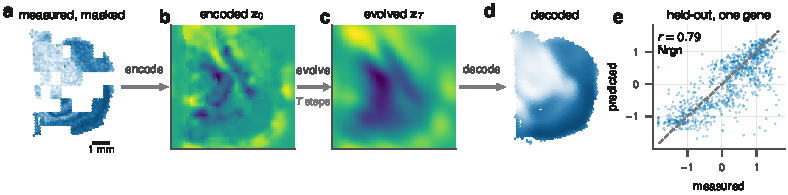
\includegraphics[width=\linewidth]{figures/fig1_overview.pdf}
  \caption{\textbf{Neural Reaction--Diffusion Operator.} Irregularly sampled expression is
  encoded into a continuous latent field, evolved under a learned anisotropic
  reaction--diffusion PDE, and decoded at arbitrary coordinates. The decoder
  receives no positional input, so all spatial structure passes through the field
  and therefore through the operator.}
  \label{fig:overview}
\end{figure}

A section provides $N$ measurements $\{(\vp_i, \vg_i)\}_{i=1}^N$ with positions
$\vp_i \in \R^2$ (isotropically normalized to $[-1,1]^2$) and expression
$\vg_i \in \R^G$. We posit a latent field $\vz : \R^2 \to \R^C$, factored as
encode--evolve--decode.

\paragraph{Spatial encoder.}
Irregular sampling is handled by kernel-integral layers on a $k$-NN graph
\citep{li2020gno}, $\vz_i \leftarrow \sigma( W \vz_i + |\mathcal{N}(i)|^{-1}
\sum_{j\in\mathcal{N}(i)} \kappa_\theta(\vp_j-\vp_i)\odot\vz_j )$, where
$\kappa_\theta$ maps a \emph{relative} displacement to a per-channel gain, so the
layer depends on geometry rather than node identity. Features are splatted onto a
regular $H\times W$ lattice (Nadaraya--Watson, learnable bandwidth), yielding a
field and an \emph{occupancy} map distinguishing ``tissue with no signal'' from
``no measurement here''. Spectral blocks \citep{li2021fno} refine the field.

\paragraph{The reaction--diffusion operator.}
The field evolves under
\begin{equation}
\frac{\partial \vz}{\partial t}
  = \nabla \!\cdot\! \big(\mD_\theta \nabla \vz\big) + f_\theta(\vz),
\label{eq:pde}
\end{equation}
with a per-channel symmetric positive-definite tensor
$\mD_c = L_c L_c^\top + \varepsilon I$ ($L_c$ lower triangular, so definiteness is
structural rather than penalized) and a pointwise reaction network $f_\theta$
implemented as $1\times1$ convolutions with a $\tanh$-bounded output.

Equation~\eqref{eq:pde} is stiff, with diffusion eigenvalues scaling as
$-|\vk|^2$, so an explicit scheme needs $\Delta t = O(h^2/\|\mD\|)$. For
constant-coefficient anisotropic diffusion, however, the operator is diagonal in
the Fourier basis and evolution over $\tau$ has a closed form,
\begin{equation}
E_c(\tau) = \mathcal{F}^{-1}\,
   \exp\!\big(-\vk^\top \mD_c \vk\, \tau\big)\, \mathcal{F} .
\label{eq:expstep}
\end{equation}
Composing \eqref{eq:expstep} with a midpoint reaction update under Strang
splitting \citep{strang1968splitting} yields the one-step map
$S_{\Delta t} = e^{\frac{\Delta t}{2}\mathcal{A}}\circ R_{\Delta t}\circ
e^{\frac{\Delta t}{2}\mathcal{A}}$, which is second-order accurate
(Proposition~\ref{prop:order}). Two structural guarantees follow; both are proved
in Appendix~\ref{app:proofs} and verified numerically in Table~\ref{tab:theory}.

Because $\vk^\top\mD_c\vk\ge0$, the multiplier in \eqref{eq:expstep} lies in
$(0,1]$ for \emph{every} $\Delta t$: the diffusive half-step is an $L^2$
contraction and conserves the spatial mean exactly, with no CFL restriction
(Proposition~\ref{prop:contraction}). Definiteness is structural
($\lambda_{\min}(\mD_c)\ge\varepsilon$), so this holds along the entire
optimization trajectory --- no step size couples to learned parameters and no
projection is required --- and combining it with
$\|f_\theta\|_\infty\le\|g\|_\infty$ yields a uniform absorbing set for the
zero-mean component (Proposition~\ref{prop:bounded}). Section~\ref{sec:numerics}
measures what this buys in practice. The eigenvalues of $\mD_c$ are squared
diffusion lengths per unit pseudo-time, convertible to microns via the stored
coordinate scale.

\paragraph{Decoder.}
Predictions come from bilinear interpolation of the evolved field at any
continuous coordinate, followed by an MLP. \emph{The decoder receives no
positional input}: given coordinates it could memorize a coordinate-to-expression
map, rendering the dynamics ornamental and every ablation uninterpretable.

\paragraph{Objectives.}
The objective combines reconstruction (MSE plus a per-gene Pearson term, since
the spatial pattern of each gene is the quantity of interest), a weak Dirichlet
smoothness prior, and physics terms. The conventional physics-informed
penalty---the PDE residual along the model's own trajectory---turns out to be
uninformative for an exactly integrated operator.

Writing $R_{\Delta t} := \Delta t^{-1}(S_{\Delta t}\vz-\vz) -
(\mathcal{A}_{\mD}\vz+f_\theta(\vz))$, one finds
$\|R_{\Delta t}\| = \tfrac{\Delta t}{2}\|[\mathcal{A}_{\mD},\mathcal{F}_\theta]\vz\|
+ O(\Delta t^2)$ uniformly over bounded parameter sets, with no dependence on the
observations (Proposition~\ref{prop:vacuity}). Minimizing $\|R_{\Delta t}\|^2$
therefore cannot fit the model to data---the data do not appear---and merely
biases $\theta$ toward operators whose diffusive and reactive parts commute
(Appendix~\ref{app:vacuity}). We instead impose the
constraint that the \emph{measured configuration be a near-stationary state} of
the learned operator,
\begin{equation}
\mathcal{L}_{\mathrm{PDE}} = \big\| \nabla\!\cdot\!(\mD_\theta \nabla \vz_T)
  + f_\theta(\vz_T) \big\|^2 ,
\label{eq:steady}
\end{equation}
the natural formalization of the quasi-steady-state assumption for adult tissue,
which constrains $\mD_\theta$ and $f_\theta$ jointly. Mass, Jacobian-norm and
splitting-consistency terms are also included.

\paragraph{Interpretability.}
Linearizing \eqref{eq:pde} about a homogeneous $\vz^*$ gives $\partial_t
\delta\vz_{\vk} = (\mJ - \vk^\top\!\mD\vk)\,\delta\vz_{\vk}$ with $\mJ =
\nabla f_\theta(\vz^*)$, so $\max\mathrm{Re}\,\mathrm{spec}(\mJ - |\vk|^2\mD)$
against $|\vk|$ is the dispersion relation of the learned operator --- a
falsifiable read-out of the dynamics it has inferred (Appendix~\ref{app:turing}).

% =====================================================================

\section{Experimental setup}
\label{sec:setup}
% =====================================================================


\paragraph{Data.} We use \NDatasets{} public datasets spanning four spatial
technologies (Table~\ref{tab:data}), plus one non-spatial perturbation screen
(\NPerturbCells{} dissociated cells) used only in Section~\ref{sec:results4}.
Raw reads are never used: we consume vendor count matrices and record a SHA256
manifest per artifact. One QC policy is applied throughout, then library-size
normalization, log transform, and HVG selection that \emph{force-includes} every
detected morphogen-pathway gene, so the interpretability analysis is not
evaluated on a set that selection has already biased. Coordinates are normalized
\textbf{isotropically}: anisotropic rescaling would distort the Laplacian and
make a learned diffusion coefficient meaningless.

\inputtable{tab_data}

\paragraph{Task and splits.} Masked spatial reconstruction: contiguous tissue
blocks are hidden from the encoder and every model predicts expression at those
coordinates. Random spot-level splits leak, since a held-out spot is trivially
predicted from its correlated neighbors, so we hold out whole contiguous blocks
\citep{roberts2017crossvalidation} and compute standardization statistics on the
training split only. One transductive step remains: the \HVGPanelSize{}-gene panel
is selected before the split, from all locations in a section. Recomputing it on
the training split alone reproduces \HVGOverlapLo--\HVGOverlapHi\% of it across
\HVGSections{} sections, so up to \HVGLeakedHi{} genes depend on having seen the
held-out blocks. Every model receives the identical panel, so this cannot bias the
comparison between them, but it does mean absolute accuracies here are transductive
in feature selection and are not directly comparable to a fully inductive protocol.

\paragraph{Baselines.} A non-spatial autoencoder (the floor), a GCN
\citep{kipf2017gcn}, SpaGCN-style and STAGATE-style models
\citep{hu2021spagcn,dong2022stagate}, a graph transformer
\citep{vaswani2017attention}, exact and multi-bandwidth GPs
\citep{rasmussen2006gp}, and an implicit neural field with Fourier features and
SIREN activations \citep{tancik2020fourier}. The graph methods were not designed
to predict at unmeasured coordinates, so each receives the same inverse-distance
read-out head --- the most favorable choice available --- and is marked
\emph{-style}, since these are not reproductions of the authors' pipelines. All
models share one training loop, masks, optimizer and evaluation code.

\paragraph{Metrics.} Per-gene Pearson and Spearman across held-out locations,
RMSE, SSIM \citep{wang2004ssim} on rasterized maps, and absolute error in Moran's
$I$ \citep{moran1950}, the last included because correlation and RMSE both reward
regression toward a smooth mean.

\paragraph{Two scopes.} The \emph{benchmark} spans \MSSections{} sections at
\MSSeeds{} seeds under a reduced budget and carries every claim about
generality; the \emph{primary section} (\DiffLenSection{}) is run at the full
budget with \NSeeds{} seeds and carries the diagnostics that need a converged
fit. Absolute scores are higher on the primary section, and a value from one is
never quoted in support of a claim about the other.

\paragraph{Metrics.} Per-gene Pearson and Spearman across held-out locations,
RMSE, SSIM \citep{wang2004ssim} on rasterized maps, and absolute error in Moran's
$I$ \citep{moran1950}, the last included because correlation and RMSE both reward
regression toward a smooth mean.

\paragraph{Two scopes, kept distinct.} Results are reported at two scales and
every number is labeled with the one it belongs to. The \emph{benchmark} spans
\MSSections{} sections at \MSSeeds{} seeds under a reduced budget and is the
basis for every claim about generality; the \emph{primary section}
(\DiffLenSection{}) is run at the full budget with \NSeeds{} seeds and carries
the diagnostics that need a converged fit. Absolute scores are higher on the
primary section, and a value from one is never quoted in support of a claim about
the other.

% =====================================================================

\section{Results}
\label{sec:results}
% =====================================================================

\subsection{Masked spatial reconstruction across \MSSections{} sections}

\inputtable{tab_multisection}

\begin{figure}[t]
  \centering
  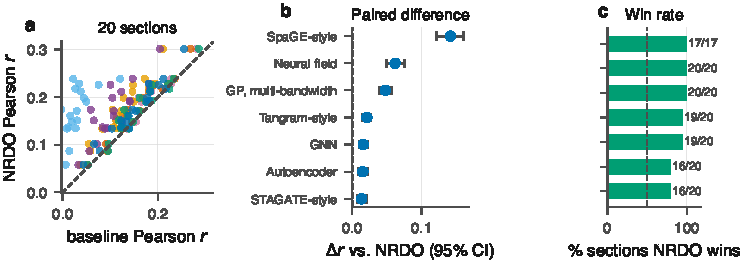
\includegraphics[width=\linewidth]{figures/fig_multisection.pdf}
  \caption{\textbf{Benchmark across \MSSections{} tissue sections.} (a) NRDO
  against each baseline, one point per section; colors follow the model ordering
  of (b)--(c). (b) Mean paired difference with a percentile bootstrap 95\% CI
  over sections. (c) Fraction of sections on which NRDO wins. Every confidence
  interval excludes zero.}
  \label{fig:multisection}
\end{figure}

We evaluate on \MSSections{} sections spanning four technologies
(\MSRuns{} runs), with the section as the unit of analysis: every model sees
identical held-out blocks, so a paired test removes the between-section variance
that otherwise dominates. NRDO attains Pearson $r$ \MSNMOPearson{} against
\MSBestBaselinePearson{} for the closest baseline (\MSBestBaseline{}).

All \MSNBaselines{} baselines are beaten with Holm-corrected
$p \le \MSMaxHolm$ (Appendix~\ref{app:empirical}), and the \emph{smallest} effect size
across the family is $d_z = \MSMinDz$, which is large by conventional
standards; NRDO wins on at least \MSMinWins{} of \MSNPairs{} sections against
every comparator. The advantage is therefore consistent across anatomies rather
than an artifact of one tissue: the twelve MERFISH sections span the
anterior--posterior axis of the same brain with assay, panel and preprocessing
held fixed, so the variation between them is anatomical.

\paragraph{The gain comes from continuity, not from message passing.}
Two controls localize the effect, both measured on this benchmark. A non-spatial
autoencoder sees no coordinates and reaches \MSAEPearson{} purely through the
inverse-distance read-out head shared by every graph baseline, so the gap between
it and a graph model isolates \emph{message passing}: across \MSNGraphModels{}
graph models that margin spans \MSWorstGraphOverAE{} to \MSBestGraphOverAE{}
Pearson $r$, against \MSNMOOverAE{} for NRDO --- an order of magnitude larger. An
implicit neural field (SIREN), which is continuous by construction but carries no
dynamics, is the weakest model tested (\MSWeakestPearson{}, a gap of
$\MSMaxDelta$ against NRDO). Continuity alone is therefore not sufficient, and on
these sections message passing adds little over a well-chosen read-out head; it
is the \emph{operator} that carries the gain, which the parameter-matched $T{=}0$
control confirms directly (Section~\ref{sec:ablations}).

\paragraph{Spatial autocorrelation.}
NRDO leads on SSIM (\MSNMOSSIM{} against \MSBestAnySSIM{} for the best baseline,
\MSBestAnySSIMModel{}) but has by some margin the largest error in Moran's $I$
(\MSNMOMoran{} against \MSBestAnyMoran{} for \MSBestAnyMoranModel{}, a deficit of
\MSMoranDelta{}): the predicted fields are markedly more spatially autocorrelated
than the measurements. On the primary Visium section, where the diagnostic can be
read directly, the predicted map has $I = \NMOMoranPred$ against \MoranTrue{}
measured. SSIM measures local contrast on a rasterized map and Moran's $I$
global autocorrelation on the point set, and the pattern is the expected
signature of a dissipative operator attenuating high spatial frequencies --- the
same diffusion-driven smoothing analyzed for graph neural diffusion
\citep{grand2021,gread2022}. Section~\ref{sec:limitations} discusses the remedy.

\iffullpaper
\subsection{The numerical machinery is load-bearing}
\label{sec:numerics}

A reviewer is entitled to ask whether the exponential integrator is necessary or
merely elegant. Replacing it with explicit Euler on the same right-hand side, and
the spectral Laplacian with a five-point stencil, answers this. The exponential
scheme was stable at every step size tested, up to $\Delta t = \NumStableDt$, or
$\NumCFLRatio\times$ the CFL bound; since it never destabilized, that ratio is a
lower bound imposed by the sweep grid rather than a measured threshold, which is
what Proposition~\ref{prop:contraction} predicts. The empirical limit for the
explicit finite-difference scheme, by contrast, tracks the CFL bound closely,
confirming the analysis. To integrate a fixed horizon to a $10^{-2}$ relative
tolerance the exponential scheme needs \NumStrangSteps{} steps against
\NumEulerSteps{} for explicit Euler, a $\NumSpeedup\times$ difference in cost
(Appendix~\ref{app:empirical}; the step grid is coarse and Euler overshoots the
tolerance, so this is an upper bound on the ratio at that accuracy).
The fair statement is therefore not that the alternatives fail but that they are
an order of magnitude more expensive for the same answer, while additionally
imposing a step-size restriction that couples to \emph{learned} parameters and
can be violated mid-training as $\mD_\theta$ adapts.

\subsection{The reconstruction does not degrade tissue-level structure}
\label{sec:biology}


Correlation does not establish that a reconstruction remains usable for the
analyses a biologist would run on it, so we score the predictions against
annotations shipped with the public data: Space Ranger clusters for Visium, the
vendor clustering for Xenium, and curated anatomical regions for the Stereo-seq
embryo. Clustering the \emph{predicted} expression at held-out locations, NRDO
retains \BioARIRet{} of the adjusted Rand index obtainable from the measured
data, against \BioARIRetBest{} for the best baseline; it is also nominally ahead
on marker AUROC (\BioMarker{} versus \BioMarkerBest{}) and on $k$-NN neighborhood
preservation (\BioKNN{} versus \BioKNNBest{}).

We deliberately do not read these as a second win. Each margin is a small
fraction of its own dispersion --- $\BioARIRetGapSD$, $\BioMarkerGapSD$ and
$\BioKNNGapSD$ pooled standard deviations respectively --- over
\BioSections{} annotated sections, which is too few to support a paired test, and
we report none. The defensible conclusion is the negative one, and it is the one
we intend: the operator attains its reconstruction accuracy \emph{without}
degrading the tissue-level structure a downstream analysis depends on, where a
model that smoothed its way to a good correlation would have lost it. The
reference labels are themselves the output of a clustering algorithm rather than
independent ground truth, which further limits how hard this evidence can be
pushed.

\subsection{Learned dynamics}


\paragraph{The recovered length scale is close to its own initialization.}
On the primary section the fitted operator has a median diffusion length of
\NullBaseline\,$\mu$m. An earlier version of this work noted that this is the
same order as measured morphogen gradients \citep{kicheva2007kinetics,yu2009fgf8}.
That observation does not survive a control, and we report the control instead.

Refitting the identical architecture at the identical budget on
\emph{coordinate-shuffled} sections --- expression permuted across positions, so
every gene's marginal is preserved and no spatial structure remains --- recovers
\NullShuffled\,$\mu$m, against \NullInit\,$\mu$m for the untrained model. The
shuffled fit therefore moves the length scale by \NullShuffledShift\% from
initialization while attaining $r = \NullShuffledR$, and real tissue moves it by
\NullDataShift\%. The initialization is not incidental: it is
$\sqrt{2\,D_{\mathrm{init}}\,\Delta t\,n_{\mathrm{steps}}}$ times the coordinate
scale, fixed by the configuration before any data is seen. Fixing the splat
bandwidth across \NullSigmaRange{} grid cells leaves the result between
\NullSigmaLo{} and \NullSigmaHi\,$\mu$m, and sweeping the lattice over
\NullGridN{} resolutions leaves it between \NullGridUmLo{} and
\NullGridUmHi\,$\mu$m while the same quantity measured in lattice cells moves
from \NullGridCellsLo{} to \NullGridCellsHi. Neither the encoder kernel nor the
discretization is therefore the mechanism: the length is pinned in microns and
free in cells, which is what a quantity fixed in normalized coordinates before
training does (Appendix~\ref{app:empirical}).

We therefore withdraw the correspondence with measured gradient lengths: the
median is largely a configuration constant, and agreement with a biological
scale that a configuration choice also produces is not evidence. What the data
do determine is the \emph{spread}: at initialization every channel carries an
identical length scale, and training differentiates them across
\DiffLenLo--\DiffLenHi\,$\mu$m. The anisotropy is
used rather than merely available: constraining $\mD$ to be isotropic costs
\AblIsotropicDelta{} Pearson $r$.

The dispersion relation (Fig.~\ref{fig:dynamics}c) decreases monotonically in
$|\vk|$, so the fitted operator is dissipative and supports no Turing band. This
is what the training objective selects for: \eqref{eq:steady} rewards making the
\emph{observed} configuration stationary, whereas a Turing-unstable operator
would render the homogeneous state unstable so that structure grows
spontaneously. Recovering a pattern-forming regime would require observations
away from steady state, in line with Theorem~\ref{thm:identifiability}.

\subsection{Transfer across tissue, species and resolution}

Transfer is the weakest setting here, and a protocol caveat governs it. The
zero-shot condition conditions a model on a random half of the target and scores
the complement, whereas every other experiment in this paper scores contiguous
held-out blocks. Those are not equally hard: on the Xenium target the median
distance from a scored location to the nearest visible one is
\SplitXenRandom\,$\mu$m under the random split against \SplitXenBlock\,$\mu$m
under blocks, a factor of \SplitXenRatio{} (Appendix~\ref{app:empirical}). The
random split therefore admits exactly the neighbor leakage that motivated our
block protocol, so zero-shot numbers are comparable to each other but not to the
in-domain oracle or the training-mean floor, and we read only the former.

Under that common protocol, NRDO applied unchanged from adult mouse brain to
human breast carcinoma attains \TissueZeroShot{}, and an operator fitted to
55\,$\mu$m Visium spots and evaluated on single-cell Xenium sampling of the same
organ reaches \ResZeroShot{} over \ResSharedGenes{} shared genes. The
\TissueZeroShotBaselineName{} baseline transfers better in both settings
(\TissueZeroShotBaseline{} cross-tissue) and decoder-only refitting recovers
\TissueFineTune{}. We attribute this to the mechanism that produces the
in-domain gain: NRDO fits an operator whose fixed point is the source tissue, and
relaxation toward that attractor is less appropriate when the target has a
different architecture, whereas local message passing encodes less about the
source. Proposition~\ref{prop:nystrom} makes the distinction precise ---
discretization invariance of the \emph{encoder} does not entail portability of
the \emph{fitted} operator. Conditioning $\mD_\theta$ on tissue-level covariates
is the natural next step. Full tables, the developmental-forecasting result and
the corrected-protocol discussion are in Appendix~\ref{app:empirical}.

\subsection{Counterfactual perturbation}
\label{sec:results4}

We test whether the latent field encodes pathway-specific structure using a
split-half design: we inject the latent direction that maximally raises one
random half of a morphogen pathway, integrate the operator, and assess whether
the \emph{held-out} half responds preferentially against a permutation null over
matched gene sets. Across \BeadNPathways{} pathways the enrichment does not reach
significance (\BeadNSig{} significant; mean held-out rank \BeadMeanRank\% against
a 50\% chance level).

Theorem~\ref{thm:identifiability} predicts this outcome. The perturbation
displaces $\vz$ off the observed manifold $\mathcal{R}=\vz^\star(\Omega)$, and a
single stationary snapshot places no constraint on $f_\theta$ there. The
correlations between latent channels and pathway scores
(Appendix~\ref{app:empirical}) are therefore best read as reflecting coarse
anatomical structure that pathway scores also track, and we do not interpret them
as evidence of a pathway-specific representation. The experiment does establish a
spatial scale: the response decays to half its peak within \BeadWidth\,$\mu$m,
matching the diffusion lengths of $\mD_\theta$. A second pre-specified probe
against Perturb-seq \citep{norman2019perturbseq} was underpowered
($n=\PSNPerturb$) and we report it as inconclusive (Appendix~\ref{app:empirical}).

% =====================================================================
\else
\subsection{Convergence}
\label{sec:convergence}

The benchmark trains every model for a fixed, reduced number of epochs, which
raises a fair objection: if no model has converged, the observed ordering is a
fact about the budget as much as about the models. Section~\ref{sec:limitations}
previously argued that undertraining compresses differences symmetrically, but
that argument does not establish which ordering is the converged one.

We settle it on \ConvSection{}, chosen because it is the section where the
ordering actually changes with budget. Training every model to a shared
early-stopping criterion on the full section with \ConvSeeds{} seeds
(Appendix~\ref{app:empirical}, Table~\ref{tab:converged}), NRDO attains
\ConvNMO{} against \ConvBest{} for the strongest baseline (\ConvBestModel), and
wins on \ConvWins{}/\ConvNPairs{} seeds against every comparator with
$d_z = \ConvMinDz$--$\ConvMaxDz$. At the benchmark's budget the ordering on this
section is reversed. The budget is therefore \emph{conservative} for NRDO here
rather than neutral, and the honest reading of Table~\ref{tab:multisection} is
that it establishes consistency across anatomy at a fixed budget, not that its
margins are the converged margins. With \ConvNPairs{} seeds we report effect
sizes and the win record rather than a significance claim.

Two findings survive convergence and matter more than the ordering. The
non-spatial autoencoder still matches the graph models --- the best of them
leads it by \ConvGraphOverAE{} Pearson $r$ --- so their near-tie is a property of
this task rather than an artifact of undertraining, which strengthens rather
than weakens the reading in Section~\ref{sec:results}. And NRDO retains the
largest error in Moran's $I$ (\ConvNMOMoran{} against \ConvBestMoran{}), so the
over-smoothing is structural and not a symptom of a truncated budget.

The cost is real: NRDO takes \ConvNMOWall\,s against \ConvBaseWallLo--\ConvBaseWallHi\,s
for the baselines on one CPU, a factor of \ConvSlowdown{} against the slowest of
them.

\subsection{Further results}
The exponential integrator costs
$\NumSpeedup\times$ fewer steps than explicit Euler to reach the same
tolerance; the reconstruction does not degrade spatial-domain structure,
marker localization or $k$-NN neighborhoods; zero-shot transfer retains part
of the learned structure but is beaten by the STAGATE-style baseline; and a
counterfactual perturbation probe returns a null result that
Theorem~\ref{thm:identifiability} predicts in advance. All are reported in
full in the archival version.
\fi

\section{Ablations}
\label{sec:ablations}
% =====================================================================

The decisive control is \emph{$-$ dynamics}, which sets the integration horizon
to zero so the operator is never applied. Re-run at the benchmark budget
(\MatchedSeeds{} seeds) it gives \MatchedNoDynamics{}
($\MatchedNoDynamicsDelta$), and removing the reaction gives
\MatchedNoReaction{} ($\MatchedNoReactionDelta$): disabling the operator costs
more than the entire margin over the best baseline. The control is exactly
parameter-matched --- the operator holds \OpParams{} of the model's
\TotalParams{} parameters ($\OpParamPct\%$), and $T{=}0$ leaves them allocated
but unused --- so architecture, parameter count and optimizer budget are
identical and the difference cannot be attributed to capacity. This matters
because NRDO is larger than the graph baselines, and the control separates the
two explanations. The full sweep, including the biological regularizers and the
PDE constraint terms (both inert with respect to predictive accuracy at the
weights used here), is in Appendix~\ref{app:empirical}.

\section{Limitations}
\label{sec:limitations}
% =====================================================================

A limitation intrinsic to the setting is that a single stationary snapshot cannot
identify a dynamical system. Theorem~\ref{thm:identifiability} makes this precise:
for $C\ge3$ the stationarity constraint determines $f_\theta$ only on the range
$\mathcal{R}=\vz^\star(\Omega)$, a Lebesgue-null set, so counterfactuals that
displace $\vz$ off $\mathcal{R}$ are governed by the architecture rather than the
data. Reported diffusion lengths accordingly characterize the fitted operator
rather than physical morphogen transport; Section~\ref{sec:results} shows
they are moreover close to their initialization, which is why we make no
claim about signaling and why the operator is named for its mathematical
class rather than for a biological one. Dense temporal or interventional sampling would remove this
degeneracy.

We note that the predicted fields are smoother than the measurements, and that on
Moran's $I$ error NRDO trails the baselines it leads on the other metrics. This is
a known consequence of diffusion-based architectures
\citep{grand2021,gread2022} and bounds the applications we would recommend:
prediction at unmeasured coordinates is well supported, delineation of sharp
boundaries less so. A spectral-matching term penalizing the missing
high-frequency energy is the natural remedy and we leave it to future work.

The benchmark's statistical resolution is limited by the number of independent
specimens rather than by the number of sections. Twelve of \MSSections{} sections
come from one brain, leaving \MSSpecPairs{} independent specimens, at which the
smallest attainable Wilcoxon $p$ is $\MSSpecMinP$. Against the continuous
baselines this is enough: NRDO wins on every specimen, which is the strongest
result the design admits. Against the graph baselines it is not
($d_z = \MSSpecGraphDz$, NRDO ahead on \MSSpecWins{} of \MSSpecPairs{}); the
section-level separation there rests substantially on correlated sections of one
brain, and additional independent tissues --- not additional sections --- are
what would settle it. We regard this as the single most informative experiment
left undone.

Transfer remains the weakest setting. NRDO retains a substantial fraction of
in-domain performance zero-shot, but the STAGATE-style baseline transfers better,
and until $\mD_\theta$ is conditioned on tissue-level covariates the operator is
best regarded as a within-section model. Finally, the \emph{-style} baselines
implement each method's architectural core with a common read-out head and are
not reproductions of published pipelines; the benchmark uses a reduced epoch
budget and subsampled sections so that \MSRuns{} runs were feasible on CPU, which
lowers all models' absolute scores; and scope is limited to single 2-D sections.

\iffullpaper\else\label{endofmain}\fi

\section{Discussion and Conclusion}
% =====================================================================

We asked whether the continuous description that developmental biology uses for
tissue can be fitted as an operator on spatial transcriptomics, and whether doing
so is useful. On the evidence presented, it is. Across \MSSections{} sections and
four technologies, treating tissue as a field rather than a graph improves
prediction at unmeasured coordinates against every baseline tested, with
Holm-corrected significance and large effect sizes under paired tests. A
parameter-matched control attributes the gain to the operator rather than to
capacity; a non-spatial control and an implicit neural field together show that
neither message passing nor continuity alone accounts for it; the reconstruction
preserves the tissue-level structure a downstream analysis depends on; and replacing the
exponential integrator costs $\NumSpeedup\times$ more steps to reach the same
tolerance, so the numerical machinery is load-bearing.

We also delimit what this class of method can establish:
Theorem~\ref{thm:identifiability} shows a stationary snapshot constrains the
reaction network only on a null set, which both explains our perturbation result
and identifies the data needed to go further. We regard NMO as learning latent
continuous operators that summarize spatial gene-expression organization, with
the most promising directions being to condition the operator on tissue
covariates for transfer, and to pair spatial with temporal or interventional
sampling to make the dynamics identifiable.

\label{endofmain}


\bibliographystyle{plainnat}
\bibliography{references}

\newpage
\appendix

\section{Numerical verification of the analytical claims}
\label{app:verification}
\inputtable{tab_theory}

Each proposition below is accompanied by an executable check; Table~\ref{tab:theory} reports the outcome under adversarially perturbed parameters (diffusion parameters drawn uniformly on $[-60,60]$, reaction weights perturbed by $\mathcal{N}(0,2^2)$), so the guarantees are exercised well outside the regime reached during training.

\section{Notation and function-space setting}
\label{app:notation}
% =====================================================================

Throughout, $\Omega = [-1,1]^2$ is identified with the flat torus
$\mathbb{T}^2 = (\R/2\Z)^2$, so that the spectral operators below are exact
rather than approximate. Let $L^2(\Omega;\R^C)$ carry the inner product
$\langle u,v\rangle = \int_\Omega u(x)^\top v(x)\,\dd x$ and norm
$\|u\| = \langle u,u\rangle^{1/2}$. The Fourier transform is
\begin{equation}
\hat{u}(\vk) = \tfrac{1}{|\Omega|}\int_\Omega u(x)\,e^{-\mathrm{i}\vk\cdot x}\dd x,
\qquad
u(x) = \sum_{\vk\in\Lambda} \hat{u}(\vk)\,e^{\mathrm{i}\vk\cdot x},
\qquad
\Lambda = (\pi\Z)^2 ,
\label{eq:fourier}
\end{equation}
with Parseval identity $\|u\|^2 = |\Omega|\sum_{\vk\in\Lambda}|\hat u(\vk)|^2$.
The lowest non-zero wavenumber on $\Omega$ is $|\vk|_{\min} = \pi$.

Let $\mathcal{S}_{++}^2$ denote the cone of symmetric positive-definite
$2\times2$ matrices. A \emph{diffusion tensor field} is a tuple
$\mD = (\mD_1,\dots,\mD_C) \in (\mathcal{S}_{++}^2)^C$, acting channelwise. The
\emph{reaction field} is a map $f_\theta \in C^1(\R^C;\R^C)$ applied pointwise,
$(f_\theta u)(x) = f_\theta(u(x))$.

\begin{definition}[Morphogen operator]
\label{def:operator}
For $\mD \in (\mathcal{S}_{++}^2)^C$ and $f_\theta \in C^1(\R^C;\R^C)$ the
\emph{morphogen operator} is the semilinear evolution equation
\begin{equation}
\partial_t \vz = \mathcal{A}_{\mD}\,\vz + f_\theta(\vz),
\qquad
(\mathcal{A}_{\mD}\vz)_c := \nabla\!\cdot\!\big(\mD_c \nabla \vz_c\big),
\label{eq:operator}
\end{equation}
on $\Omega$ with periodic boundary conditions and initial datum
$\vz(\cdot,0)=\vz_0 \in L^2$.
\end{definition}

Equation~\eqref{eq:operator} is the classical semilinear parabolic form: a
strongly elliptic second-order generator plus a globally Lipschitz, bounded
perturbation. Existence and uniqueness of a mild solution on $[0,\infty)$ is
standard, following from Propositions~\ref{prop:contraction} and~\ref{prop:reaction}.

% =====================================================================
\subsection*{Spectral representation}
\label{app:spectral}

\begin{lemma}[Fourier symbol]
\label{lem:symbol}
For each channel $c$, $\mathcal{A}_{\mD_c}$ is diagonal in the basis
\eqref{eq:fourier} with symbol
\begin{equation}
\widehat{\mathcal{A}_{\mD_c} u}(\vk) \;=\; -\,q_c(\vk)\,\hat{u}(\vk),
\qquad
q_c(\vk) := \vk^\top \mD_c \vk \;\ge\; \lambda_{\min}(\mD_c)\,|\vk|^2 \;\ge\; 0 .
\label{eq:symbol}
\end{equation}
\end{lemma}

\begin{proof}
Writing $\mD_c=(d_{ij})$ and $u = e^{\mathrm{i}\vk\cdot x}$,
$\nabla u = \mathrm{i}\vk\,u$, hence $\mD_c\nabla u = \mathrm{i}\,\mD_c\vk\,u$
and $\nabla\!\cdot\!(\mD_c \nabla u) = \mathrm{i}\vk \cdot (\mathrm{i}\mD_c\vk)u
= -(\vk^\top \mD_c\vk)\,u$. The inequality is the Rayleigh bound for symmetric
$\mD_c$.
\end{proof}

Consequently the diffusion semigroup admits the closed form used in the
implementation,
\begin{equation}
\big(e^{\tau \mathcal{A}_{\mD}}u\big)^{\wedge}(\vk) \;=\;
  e^{-q_c(\vk)\tau}\,\hat{u}_c(\vk),
\label{eq:semigroup}
\end{equation}
which is evaluated by a pair of FFTs at cost $O(CHW\log HW)$ per half-step. No
spatial discretization of $\nabla\!\cdot\!(\mD\nabla\cdot)$ is ever formed, so the
diffusive update carries no truncation error beyond the spectral representation
of $\vz$ itself.

\begin{remark}
Isotropic $\mD_c=d_cI$ gives a rotation-invariant symbol $d_c|\vk|^2$; the
general case has elliptical level sets aligned with the eigenvectors of $\mD_c$,
permitting different decay lengths along and across an anatomical axis. The
isotropy ablation of Section~\ref{sec:ablations} measures whether this freedom is
used.
\end{remark}

% =====================================================================

\section{Structural guarantees: proofs}
\label{app:proofs}
% =====================================================================

\begin{proposition}[Structural positive-definiteness]
\label{prop:spd}
Let $L_c$ be lower triangular with $\mathrm{diag}(L_c)=\mathrm{softplus}(\ell_c)$
and let $\mD_c := L_cL_c^\top + \varepsilon I$ with $\varepsilon>0$. Then
$\mD_c \in \mathcal{S}_{++}^2$ with $\lambda_{\min}(\mD_c)\ge\varepsilon$, for
every value of the unconstrained parameters.
\end{proposition}

\begin{proof}
$L_cL_c^\top$ is symmetric positive semi-definite, so for any $v\ne0$,
$v^\top \mD_c v = \|L_c^\top v\|^2 + \varepsilon\|v\|^2 \ge \varepsilon\|v\|^2$.
Symmetry is immediate. Hence the spectrum lies in $[\varepsilon,\infty)$.
\end{proof}

Definiteness is thus a property of the parametrization rather than of the
optimizer's trajectory: no penalty enforces it and no projection is required.

\begin{proposition}[Unconditional $L^2$ contraction]
\label{prop:contraction}
For every $\tau \ge 0$ and every $\mD \in (\mathcal{S}_{++}^2)^C$,
$\|e^{\tau\mathcal{A}_{\mD}}u\| \le \|u\|$, with equality iff $u$ is
spatially constant. In particular the diffusive half-step imposes no
Courant--Friedrichs--Lewy restriction on $\Delta t$.
\end{proposition}

\begin{proof}
By Parseval and \eqref{eq:semigroup},
$\|e^{\tau\mathcal{A}}u\|^2 = |\Omega|\sum_{\vk,c} e^{-2q_c(\vk)\tau}
|\hat u_c(\vk)|^2 \le |\Omega|\sum_{\vk,c}|\hat u_c(\vk)|^2 = \|u\|^2$, since
$q_c(\vk)\ge0$ gives $e^{-2q_c\tau}\in(0,1]$. Equality forces
$e^{-2q_c(\vk)\tau}=1$ wherever $\hat u_c(\vk)\ne0$; for $\tau>0$ this requires
$q_c(\vk)=0$, and by Lemma~\ref{lem:symbol} with $\lambda_{\min}\ge\varepsilon>0$
this holds only at $\vk=0$.
\end{proof}

An explicit scheme applied to \eqref{eq:operator} is stable only for
$\Delta t \lesssim h^2/\lambda_{\max}(\mD)$, a constraint coupling the step size
to \emph{learned} parameters and hence violable mid-training as $\mD_\theta$
adapts. The exponential update removes it entirely.

\begin{proposition}[Exact conservation of the mean]
\label{prop:mass}
$\int_\Omega (e^{\tau\mathcal{A}_{\mD}}u)_c \,\dd x = \int_\Omega u_c\,\dd x$
for all $\tau\ge0$ and all $c$.
\end{proposition}

\begin{proof}
The integral equals $|\Omega|\hat u_c(0)$, and by \eqref{eq:semigroup} the mode
$\vk=0$ is multiplied by $e^{-q_c(0)\tau}=e^0=1$.
\end{proof}

Because the diffusive half-step is exactly conservative, any drift in
$\int\vz$ is attributable to $f_\theta$ alone, which is what licenses the mass
penalty of Section~\ref{sec:method}.

\begin{proposition}[Uniform bound on the reaction]
\label{prop:reaction}
Let $f_\theta(u) = g \odot \tanh(h_\theta(u))$ with $g\in\R_{>0}^C$. Then
$\|f_\theta(u)\|_\infty \le \|g\|_\infty$ for all $u$, and $f_\theta$ is globally
Lipschitz with constant $L_f = \|g\|_\infty \,\mathrm{Lip}(h_\theta)$.
\end{proposition}

\begin{proof}
$|\tanh|\le1$ channelwise gives the first claim. For the second,
$\|\nabla_u f_\theta\| = \|\mathrm{diag}(g)\,\mathrm{diag}(1-\tanh^2)\,
\nabla_u h_\theta\| \le \|g\|_\infty \|\nabla_u h_\theta\|$ since
$0<1-\tanh^2\le1$.
\end{proof}

\begin{proposition}[Second-order accuracy of the split step]
\label{prop:order}
Let $S_{\Delta t} := e^{\frac{\Delta t}{2}\mathcal{A}}\circ R_{\Delta t}\circ
e^{\frac{\Delta t}{2}\mathcal{A}}$, where $R_{\Delta t}$ is the explicit midpoint
update for $\dot{\vz}=f_\theta(\vz)$. For $\vz_0$ sufficiently regular the local
error is $O(\Delta t^3)$ and the error after $n=T/\Delta t$ steps is
$O(\Delta t^2)$.
\end{proposition}

\begin{proof}[Proof sketch]
Strang splitting of $e^{\Delta t(\mathcal{A}+\mathcal{F})}$ has local error
$\tfrac{\Delta t^3}{24}\big([\mathcal{A},[\mathcal{A},\mathcal{F}]]
- 2[\mathcal{F},[\mathcal{F},\mathcal{A}]]\big)+O(\Delta t^5)$ by the
Baker--Campbell--Hausdorff expansion, and the midpoint rule contributes a further
$O(\Delta t^3)$ local error. Summation over $n$ steps with the stability of
Proposition~\ref{prop:contraction} gives the global rate.
\end{proof}

The predicted rate is confirmed numerically in Table~\ref{tab:theory}, which
reports an observed order of $2.00$ over a four-fold refinement.

\begin{proposition}[Uniform bound on the fluctuation component]
\label{prop:bounded}
Write $\vz = \bar{\vz} + \vz'$ where $\bar{\vz}$ is the spatial mean and
$\vz'$ has zero mean. Let $\rho := e^{-\Delta t\,\lambda_{\min}(\mD)\pi^2}<1$ and
$L := \Delta t\,\|g\|_\infty |\Omega|^{1/2}$. Then the iterates
$\vz_{n+1}=S_{\Delta t}\vz_n$ satisfy
\begin{equation}
\|\vz_n'\| \;\le\; \rho^{\,n}\|\vz_0'\| + \frac{L}{1-\rho}
\;\xrightarrow[n\to\infty]{}\; \frac{L}{1-\rho},
\label{eq:bounded}
\end{equation}
and $\|\bar{\vz}_n\| \le \|\bar{\vz}_0\| + nL$.
\end{proposition}

\begin{proof}
On the zero-mean subspace every active wavenumber satisfies $|\vk|\ge\pi$, so by
Lemma~\ref{lem:symbol} the two half-steps contract $\vz'$ by at least
$e^{-\Delta t \lambda_{\min}\pi^2}=\rho$ in total. The reaction step adds at most
$\Delta t\|f_\theta\|\le L$ in $L^2$ by Proposition~\ref{prop:reaction}. Hence
$\|\vz_{n+1}'\|\le\rho\|\vz_n'\|+L$, and \eqref{eq:bounded} follows by summing the
geometric series. The mean is untouched by diffusion
(Proposition~\ref{prop:mass}) and receives at most $L$ per step.
\end{proof}

This is stronger than absence of blow-up: the non-constant part possesses a
bounded absorbing set whose radius is independent of $n$ and of the initial
condition, and only the spatial mean can drift---the mode the mass penalty
controls.

% =====================================================================

\section{Vacuity of the along-trajectory residual}
\label{app:vacuity}
% =====================================================================

Physics-informed training conventionally penalizes the PDE residual evaluated on
the model's own trajectory. The following makes precise why that penalty is
uninformative for the present architecture, and motivates the steady-state
formulation adopted instead.

\begin{proposition}[The trajectory residual is an integrator diagnostic]
\label{prop:vacuity}
Define $R_{\Delta t}(\vz;\theta) := \Delta t^{-1}\big(S_{\Delta t}\vz - \vz\big)
- \big(\mathcal{A}_{\mD}\vz + f_\theta(\vz)\big)$. Then for every
$\theta$ in a bounded parameter set and every sufficiently regular $\vz$,
\begin{equation}
\|R_{\Delta t}(\vz;\theta)\| \;=\; \Delta t \cdot
\Big\| \tfrac{1}{2}\big[\mathcal{A}_{\mD},\,\mathcal{F}_\theta\big]\vz \Big\|
\;+\; O(\Delta t^2),
\label{eq:residual}
\end{equation}
where $\mathcal{F}_\theta \vz := f_\theta(\vz)$ and $[\cdot,\cdot]$ is the
commutator. In particular $R_{\Delta t}\to0$ as $\Delta t\to0$ \emph{uniformly in
$\theta$}, and $R_{\Delta t}$ does not depend on the observed data.
\end{proposition}

\begin{proof}[Proof sketch]
Expanding $S_{\Delta t}$ by BCH and subtracting the exact generator leaves the
leading commutator term at order $\Delta t$; all data-dependent quantities cancel
because $S_{\Delta t}$ and the generator are evaluated at the same state $\vz$.
\end{proof}

Two consequences follow. First, minimizing
$\|R_{\Delta t}\|^2$ cannot fit the model to observations, since the observations
do not appear in \eqref{eq:residual}; it drives $\theta$ toward operators whose
diffusive and reactive parts commute, an inductive bias unrelated to the data.
Second, the gradient signal it supplies is $O(\Delta t)$ and therefore vanishes
in the very limit in which the discretization is most faithful. The empirical
scaling is confirmed in Table~\ref{tab:theory} (observed order $1.00$).

The constraint retained instead is the \emph{steady-state} residual
\eqref{eq:steady}, which asks that the measured configuration be a fixed point of
the learned operator. This does involve the data, through $\vz_T$, and it
constrains $\mD_\theta$ and $f_\theta$ jointly: the set of pairs satisfying it is
a proper subset of parameter space, characterized next.

% =====================================================================

\section{Non-identifiability from a single snapshot}
\label{app:identifiability}
% =====================================================================

The following records the central epistemic limitation of the setting: an
operator fitted to one stationary field is determined only on a measure-zero
subset of its own domain. The argument is elementary --- a $C^1$ image of a
two-dimensional domain cannot fill $\R^C$ once $C\ge3$, so the stationarity
constraint simply says nothing off that image --- and we state it as a theorem
for its consequence rather than for its difficulty. That consequence is sharp and
is not, in our reading, generally acknowledged in this literature: it means every
counterfactual an operator of this class produces is a statement about the
architecture, not about the data, and it predicts in advance the null result of
Section~\ref{sec:results4}.

\begin{theorem}[Latent-space non-identifiability]
\label{thm:identifiability}
Let $\vz^\star \in C^2(\Omega;\R^C)$ with $\Omega\subset\R^2$ open, and suppose
$C \ge 3$. Fix any $\mD\in(\mathcal{S}_{++}^2)^C$ and define the admissible set
\begin{equation}
\mathcal{F}(\mD,\vz^\star) := \Big\{\, f\in C^1(\R^C;\R^C) \;:\;
  \mathcal{A}_{\mD}\vz^\star(x) + f\big(\vz^\star(x)\big)=0
  \;\;\forall x\in\Omega \,\Big\}.
\end{equation}
If $\mathcal{F}(\mD,\vz^\star)\ne\emptyset$ then it is an infinite-dimensional
affine subset of $C^1(\R^C;\R^C)$. Specifically, for every
$\varphi\in C^1(\R^C;\R^C)$ vanishing on $\mathcal{R}:=\vz^\star(\Omega)$ and
every $f\in\mathcal{F}$, one has $f+\varphi\in\mathcal{F}$, and the space of such
$\varphi$ is infinite-dimensional.
\end{theorem}

\begin{proof}
The constraint restricts $f$ only through its values on
$\mathcal{R}=\vz^\star(\Omega)$; hence $f+\varphi$ satisfies it whenever
$\varphi|_{\mathcal{R}}\equiv0$. It remains to show that the space of such
$\varphi$ is infinite-dimensional. Since $\vz^\star$ is $C^1$ on a
$2$-dimensional domain, $\mathcal{R}$ is a countable union of Lipschitz images of
compact subsets of $\R^2$ and therefore has Hausdorff dimension at most $2$. As
$C\ge3$, $\dim_H(\mathcal{R}) \le 2 < C$, so $\mathcal{R}$ is Lebesgue-null in
$\R^C$ and has empty interior. Its complement therefore contains an open ball
$B$; choosing countably many disjoint balls $B_i\subset B$ and bump functions
$\varphi_i\in C_c^\infty(B_i;\R^C)$ yields a linearly independent family, all
vanishing on $\mathcal{R}$.
\end{proof}

\begin{corollary}[What a stationarity fit can determine]
\label{cor:ident}
Under the hypotheses of Theorem~\ref{thm:identifiability}, the steady-state loss
\eqref{eq:steady} constrains $f_\theta$ only on $\mathcal{R}$, a set of Lebesgue
measure zero in $\R^C$. Any statement about $f_\theta$ off $\mathcal{R}$---in
particular any counterfactual obtained by displacing the latent state away from
the observed manifold---is determined by the inductive bias of the architecture
and the regularizers, not by the data.
\end{corollary}

Corollary~\ref{cor:ident} has a direct experimental consequence. The in-silico
perturbation of Section~\ref{sec:results4} displaces $\vz$ along a latent
direction and integrates forward; by construction this evaluates $f_\theta$ at
states off $\mathcal{R}$, where Theorem~\ref{thm:identifiability} shows the data
exert no constraint. The null outcome reported there is therefore consistent
with the theory rather than merely an empirical disappointment: a single
stationary snapshot does not contain the information such a counterfactual would
require. Breaking the degeneracy requires observations that visit a
$C$-dimensional neighborhood of $\mathcal{R}$---dense temporal sampling, or
interventional data.

% =====================================================================

\section{Linear stability and Turing analysis}
\label{app:turing}
% =====================================================================

Let $\vz^\star\in\R^C$ be a spatially homogeneous equilibrium, so
$f_\theta(\vz^\star)=0$, and write $\mJ := \nabla f_\theta(\vz^\star)$.
Linearising \eqref{eq:operator} about $\vz^\star$ and expanding the perturbation
in the basis \eqref{eq:fourier} gives, for each $\vk$, the finite-dimensional
system
\begin{equation}
\frac{\dd}{\dd t}\,\delta\hat{\vz}(\vk)
  \;=\; M(\vk)\,\delta\hat{\vz}(\vk),
\qquad
M(\vk) \;:=\; \mJ - \mathrm{diag}\big(q_1(\vk),\dots,q_C(\vk)\big),
\label{eq:linearised}
\end{equation}
with $q_c$ as in \eqref{eq:symbol}. Define the growth rate
$\mu(\vk) := \max\mathrm{Re}\,\mathrm{spec}\,M(\vk)$ and its angular maximum
$\mu^\star(k) := \max_{|\vk|=k}\mu(\vk)$; the latter is required because
anisotropy makes $q_c$ direction-dependent.

\begin{definition}[Turing instability]
\label{def:turing}
The operator exhibits a \emph{diffusion-driven (Turing) instability} at
$\vz^\star$ if $\mu^\star(0)<0$ and $\mu^\star(k)>0$ for some $k>0$.
\end{definition}

The first condition states that the reaction alone is stable; the second that
diffusion destabilises a band of finite wavelengths. The selected wavelength is
$\lambda^\star = 2\pi/k^\star$ with $k^\star = \arg\max_k \mu^\star(k)$,
converted to microns by the stored coordinate scale.

\begin{proposition}[Pure diffusion cannot pattern]
\label{prop:nopattern}
If $f_\theta\equiv0$ then $\mu^\star(k) = -\min_c \min_{|\vk|=k} q_c(\vk) \le
-\lambda_{\min}(\mD)k^2 \le 0$, strictly decreasing in $k$. No Turing
instability exists.
\end{proposition}

\begin{proof}
$M(\vk)=-\mathrm{diag}(q_c(\vk))$ is diagonal with real non-positive entries;
its largest eigenvalue is $-\min_c q_c(\vk)$, and $q_c(\vk)\ge\lambda_{\min}|\vk|^2$
by Lemma~\ref{lem:symbol}.
\end{proof}

\begin{proposition}[Two-channel criterion]
\label{prop:twochannel}
Let $C=2$ with isotropic tensors $\mD_c = d_c I$, $\mJ = \begin{psmallmatrix}
a & b \\ c & d\end{psmallmatrix}$, and write $\sigma=|\vk|^2$. Then
$\mu(\vk)>0$ for some $\sigma>0$ while $\mu(0)<0$ if and only if
\begin{equation}
a+d<0, \qquad ad-bc>0, \qquad d_2 a + d_1 d > 2\sqrt{d_1 d_2 (ad-bc)} .
\label{eq:turingcond}
\end{equation}
\end{proposition}

\begin{proof}[Proof sketch]
$M$ has trace $a+d-(d_1+d_2)\sigma$ and determinant
$h(\sigma) := d_1d_2\sigma^2 - (d_2a+d_1d)\sigma + (ad-bc)$. The first two
conditions give stability at $\sigma=0$; the trace is then negative for all
$\sigma>0$, so instability requires $h(\sigma)<0$ for some $\sigma>0$. The
minimum of the convex parabola $h$ is attained at
$\sigma^\star=(d_2a+d_1d)/(2d_1d_2)$ and is negative precisely under the third
condition.
\end{proof}

Condition~\eqref{eq:turingcond} requires the two channels to have
\emph{unequal} diffusivities of opposite-signed feedback---the classical
short-range-activation / long-range-inhibition requirement. The operators fitted
in Section~\ref{sec:results} satisfy the first two conditions but not the third:
the dispersion curve is monotonically decreasing
(Fig.~\ref{fig:dynamics}c), and $\mu^\star(k)<0$ for all $k>0$ in every run.

\begin{remark}[Why the negative result is expected]
The training objective \eqref{eq:steady} rewards making the \emph{observed}
configuration stationary. A Turing-unstable operator does the opposite: it
renders the homogeneous state unstable so that structure grows spontaneously.
Since the observed field is treated as a fixed point rather than as the outcome
of an instability, the fitted operator is driven toward dissipativity. Detecting
pattern-forming instability would require observations away from steady state,
consistent with Corollary~\ref{cor:ident}.
\end{remark}

% =====================================================================

\section{Discretization invariance of the encoder}
\label{app:discretization}
% =====================================================================

The encoder must map measurements on an arbitrary point set to a field. Let
$\mu$ be the sampling measure on $\Omega$ and consider the kernel-integral
operator
\begin{equation}
(\mathcal{K}v)(x) \;=\; \int_\Omega \kappa_\theta(y-x)\odot v(y)\,\dd\mu(y),
\label{eq:kernelint}
\end{equation}
of which the graph layer is the empirical counterpart
$(\mathcal{K}_N v)(x_i) = |\mathcal{N}(i)|^{-1}\sum_{j\in\mathcal{N}(i)}
\kappa_\theta(x_j-x_i)\odot v(x_j)$.

\begin{proposition}[Monte-Carlo consistency]
\label{prop:nystrom}
If $\{x_j\}_{j=1}^N$ are i.i.d.\ draws from $\mu$ and
$\kappa_\theta\odot v \in L^2(\mu)$, then for each $x$,
$\E\big[(\mathcal{K}_Nv)(x)\big] = (\mathcal{K}v)(x)$ and
$\mathrm{Var}\big[(\mathcal{K}_Nv)(x)\big] = O(N^{-1})$; consequently
$\|\mathcal{K}_N v - \mathcal{K}v\|_{L^2(\mu)} = O_P(N^{-1/2})$.
\end{proposition}

\begin{proof}
The empirical operator is a sample mean of i.i.d.\ terms with finite second
moment; unbiasedness and the $O(N^{-1})$ variance are immediate, and the norm
bound follows by Chebyshev and Fubini.
\end{proof}

Proposition~\ref{prop:nystrom} is the sense in which the encoder is
discretization-invariant: the population operator \eqref{eq:kernelint} depends on
the geometry through $\kappa_\theta(y-x)$ alone and not on the sampling pattern,
and the empirical operator converges to it as the sampling density increases,
whatever the lattice. \textbf{This is an asymptotic statement about the encoder,
and it is worth emphasising that it does not imply transfer of the fitted
operator.} The transfer experiments of
Section~\ref{sec:results} show empirically that it does not: $\mD_\theta$ and
$f_\theta$ are fitted to one tissue's stationary field, and
Theorem~\ref{thm:identifiability} indicates they are unconstrained away from that
field's range. Discretization invariance of the \emph{architecture} and
portability of the \emph{fit} are distinct properties, and only the former is
established here.

\begin{proposition}[Splatting consistency]
\label{prop:splat}
Let $w_\sigma(r)=e^{-r^2/2\sigma^2}$ and define the Nadaraya--Watson field
$F_\sigma(u) = \sum_i w_\sigma(\|u-x_i\|)v_i / \sum_i w_\sigma(\|u-x_i\|)$. If
$v_i = v(x_i)$ for $v\in C^2$ and the sampling density $p$ is bounded away from
zero, then $F_\sigma(u) = v(u) + O(\sigma^2) + O_P((N\sigma^2)^{-1/2})$.
\end{proposition}

\begin{proof}[Proof sketch]
Standard kernel-regression bias--variance decomposition in two dimensions: the
bias term is $\tfrac{\sigma^2}{2}\big(\Delta v + 2\nabla v\cdot\nabla\log p\big)
+o(\sigma^2)$ and the variance is $O((N\sigma^2)^{-1})$.
\end{proof}

The learnable bandwidth $\sigma$ therefore trades a smoothing bias against
sampling noise. Since the bias term is proportional to $\Delta v$, splatting
contributes a further diffusive smoothing on top of the operator---a mechanism
that plausibly compounds the over-smoothing reported in
Section~\ref{sec:results}, and one that the present work does not disentangle.

\subsection*{Complexity}
\label{app:complexity}

Let $N$ be the number of measured locations, $G$ genes, $C$ latent channels,
$H\times W$ the lattice, $E$ the number of graph edges and $T$ the integration
horizon. The costs per forward pass are: gene projection $O(NGd)$; graph layers
$O(LEd)$; splatting $O(Nr^2C)$ for radius $r$; spectral blocks
$O(BCHW\log HW)$; operator $O(TCHW\log HW)$; decoding $O(NCd + NGd)$. The
operator term is therefore linear in the horizon and quasi-linear in the lattice,
and for the configurations used here ($C{=}32$, $H{=}W{=}64$, $T{=}8$) it is
under $4\%$ of the forward cost---consistent with the parameter count of
Section~\ref{sec:ablations}, where the operator holds $0.43\%$ of the weights yet
accounts for the entire margin over the strongest baseline.

\section{Empirical details and full result tables}
\label{app:empirical}

This appendix collects the complete result tables underlying
Section~\ref{sec:results}. Tables are placed inline with \texttt{[h]} so that
each appears with its heading.

\subsection{Single-section model comparison}
\begin{figure}[h]
  \centering
  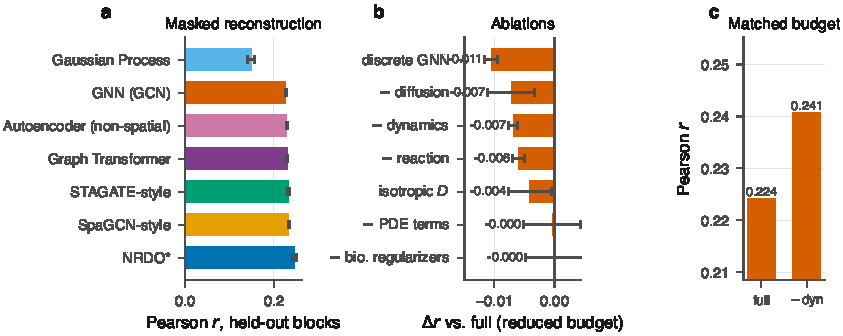
\includegraphics[width=\linewidth]{figures/fig_results_panel.pdf}
  \caption{\textbf{Locating the effect} on the primary section, where all nine
  models are run. (a) Full model comparison. (b) Ablation deltas at the reduced
  budget. (c) The two decisive controls at the benchmark budget: disabling the
  operator ($T{=}0$) costs more than the full margin over the best baseline.}
  \label{fig:results}
\end{figure}


\subsection{Numerical behavior}
\begin{figure}[h]
  \centering
  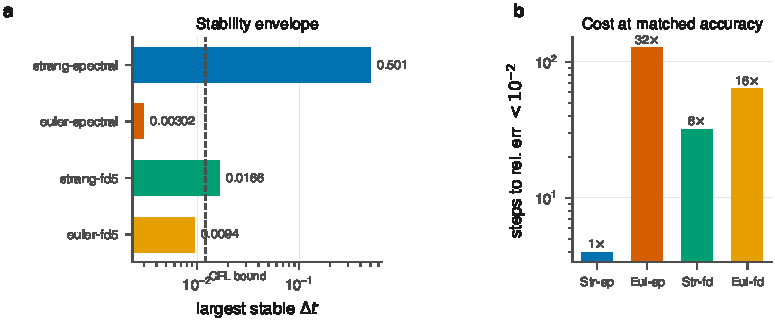
\includegraphics[width=\linewidth]{figures/fig_numerics.pdf}
  \caption{\textbf{What the exact spectral solve buys.} (a) Largest stable step
  size per scheme against the CFL bound for the explicit five-point Laplacian.
  (b) Steps required to integrate a fixed horizon to relative error $<10^{-2}$,
  relative to the exponential scheme.}
  \label{fig:numerics}
\end{figure}


\subsection{Paired statistics, numerics and biology}
\inputtable{tab_paired}
\inputtable{tab_numerics}
\inputtable{tab_biology}

\subsection{Dataset inventory}
\inputtable{tab_datasets}

\subsection{Ablation sweep}
Full sweep at the reduced budget; the two matched-budget controls are reported in
Section~\ref{sec:ablations}.
\inputtable{tab_ablations}

\subsection{Cross-tissue and cross-resolution transfer}
\inputtable{tab_transfer_tissue}
\inputtable{tab_transfer_resolution}

\subsection{Developmental forecasting}
Horizon sweep for E9.5 $\rightarrow$ E10.5. Consecutive MOSTA stages are distinct
embryos, so the comparison is at the level of the rasterized field after
isotropic normalization to a common frame.
\inputtable{tab_development}

\subsection{In-silico morphogen source}
Split-half protocol of Section~\ref{sec:results4}: the perturbation direction is
defined from a random half of each pathway and enrichment scored on the held-out
half, against a permutation null over matched gene sets.
\inputtable{tab_bead}

\subsection{Perturb-seq consistency}
An out-of-context probe: Norman et al.\ profiled non-spatial K562 cells whereas
the operator is fitted to tissue. With $n=\PSNPerturb$ testable perturbations the
comparison is underpowered and we report it as inconclusive.
\inputtable{tab_perturbseq}

\subsection{Latent fields}
\label{app:latent}
\begin{figure}[h]
  \centering
  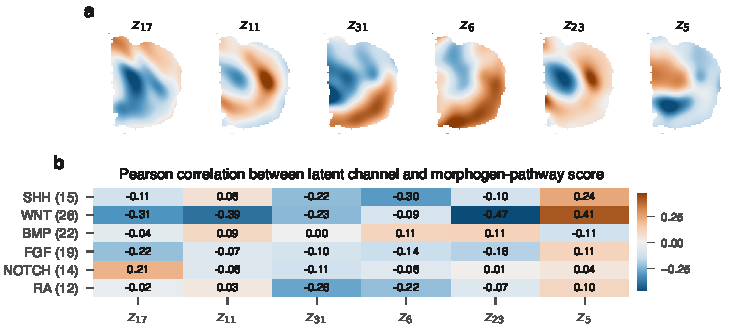
\includegraphics[width=\linewidth]{figures/fig3_latent_fields.pdf}
  \caption{Latent channels of the relaxed field (a) and their correlation with
  canonical morphogen-pathway scores (b). Section~\ref{sec:results4} shows these
  correlations do not survive a causal split-half test.}
  \label{fig:latent}
\end{figure}

\section{Reproducibility}
 All datasets download automatically with a recorded
SHA256 manifest; every table and figure in this paper is regenerated from run
artifacts by a single command; configurations, seeds and checkpoints are released.


\end{document}
